\documentclass[../thesis.tex]{subfiles}

\begin{document}

\chapter{System Architecture}

\section{Introduction}

In the \autoref{sec:layers} and \autoref{sec:responsibilities}, the logical layering and the responsibilities of the components were introduced but how they fit together and work in harmony is still a mystery. In this chapter, I will put the pieces of the puzzle together by discussing of the actual architecture of the system and its behaviours with increasing levels of detail. 


\section{Top-level architecture}

The top-level architecture is a simplified architecture where many low-level components are being grouped together and treated as a singular composite component. It is shown in the figure \ref{fig:toplevel}. The following components in the top-level architecture are composite component:

\begin{itemize}
	\item Remote Sensing (See \autoref{sec:remoteSensing})
	\item Backend (See \autoref{sec:backend})
	\item Frontend (See \autoref{sec:frontend})
	\item Real-time (See \autoref{sec:realtime})
	\item Governor (See \autoref{sec:governor})
\end{itemize}

\newgeometry{bottom=1.5cm}
\begin{figure}[!ht]
	\centering
	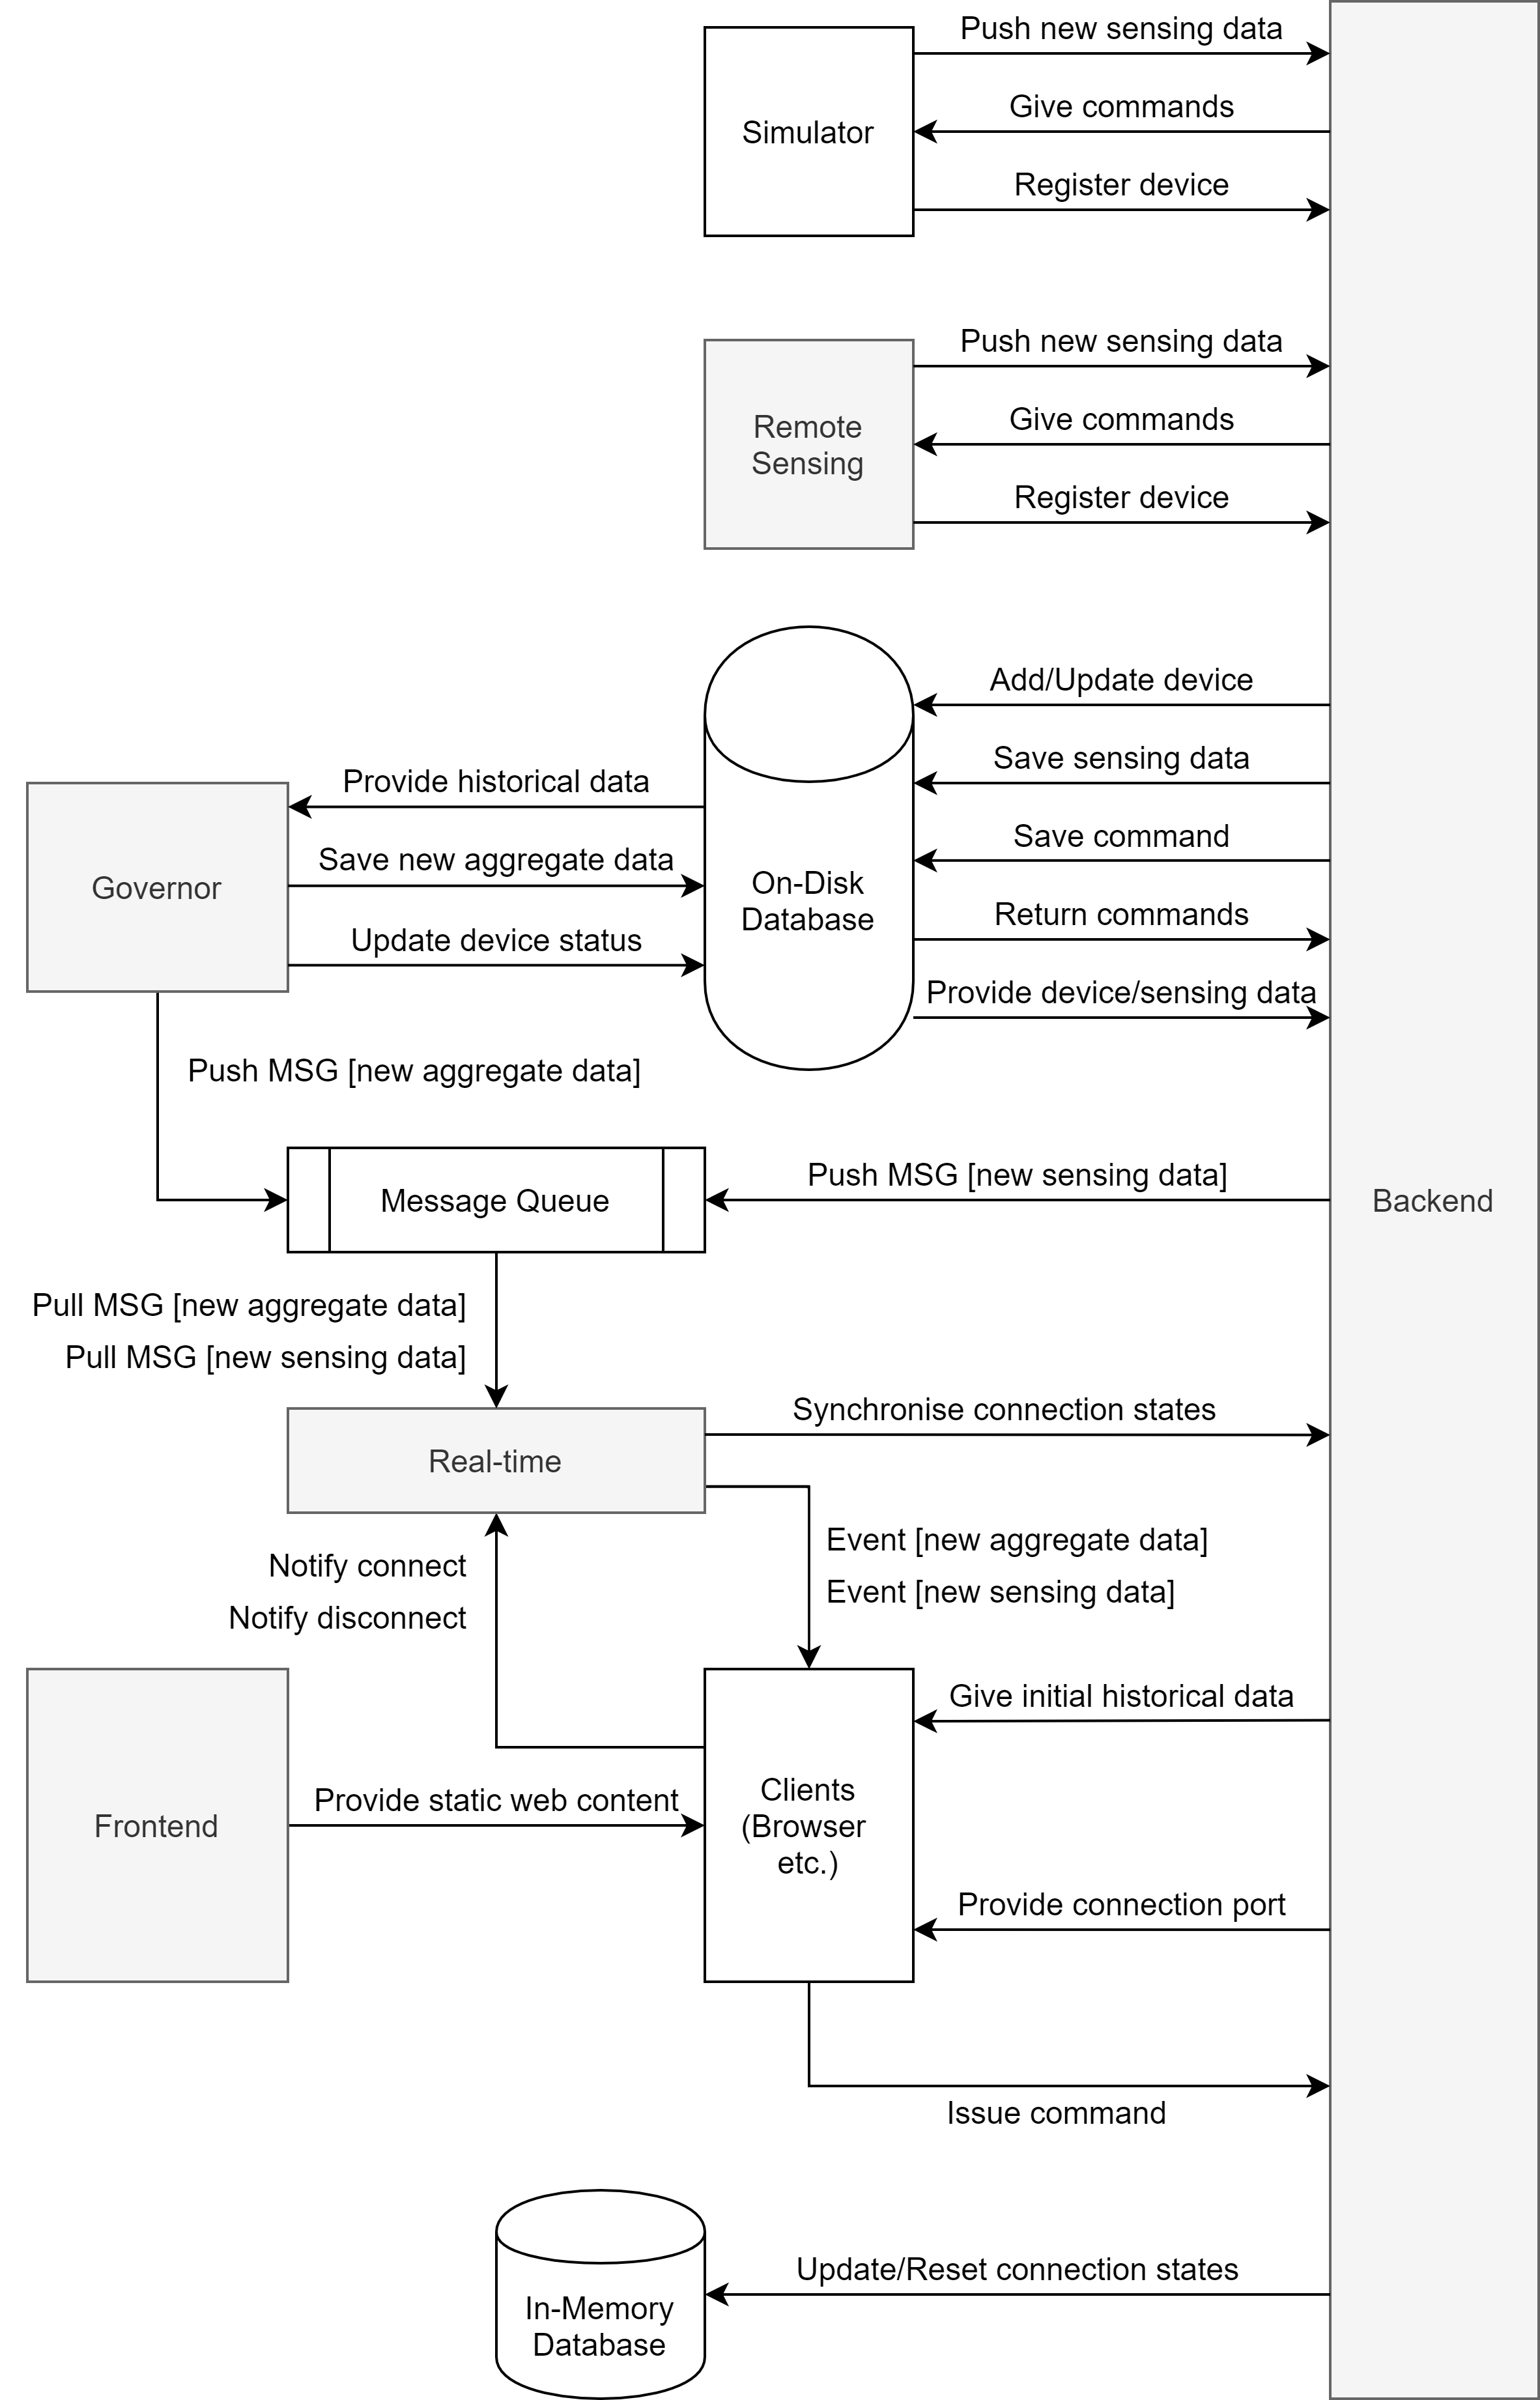
\includegraphics[width=\linewidth]{c4-toplevel.png}
	\caption{Top-level architecture of the proposed system.}
	\label{fig:toplevel}
\end{figure}
\restoregeometry

\subsection{Initialisation}

The initialisation process is referring to a device in the remote sensing composite component such as a microcontroller attempting to connect with the server before it can send data and receive commands. When a microcontroller is initialising, it sends a register device request to the backend and then wait for the reply from the backend. Once the request is received by the backend, it tries to find a matching device in the database. If found, then it updates the device status to online. Otherwise, it generates a new device ID, creates a representation of the new device in the database, and set the device status to online. Finally, the backend notifies the microcontroller by returning a response to the initial device registration request, and the intialisation sequence is complete. The figure \ref{fig:init} shows the flow of the initialisation process and the relevant function calls shown in the top-level architecture.

The initialisation process achieves two goals, the first goal is letting the backend knows the device is online and ready to transmit data, and the second goal is getting a unique ID so that it can be identified during the data transmission phase. Once the initialisation process is finished, the microcontroller is ready to transmit data. 

\begin{figure}[!ht]
	\centering
	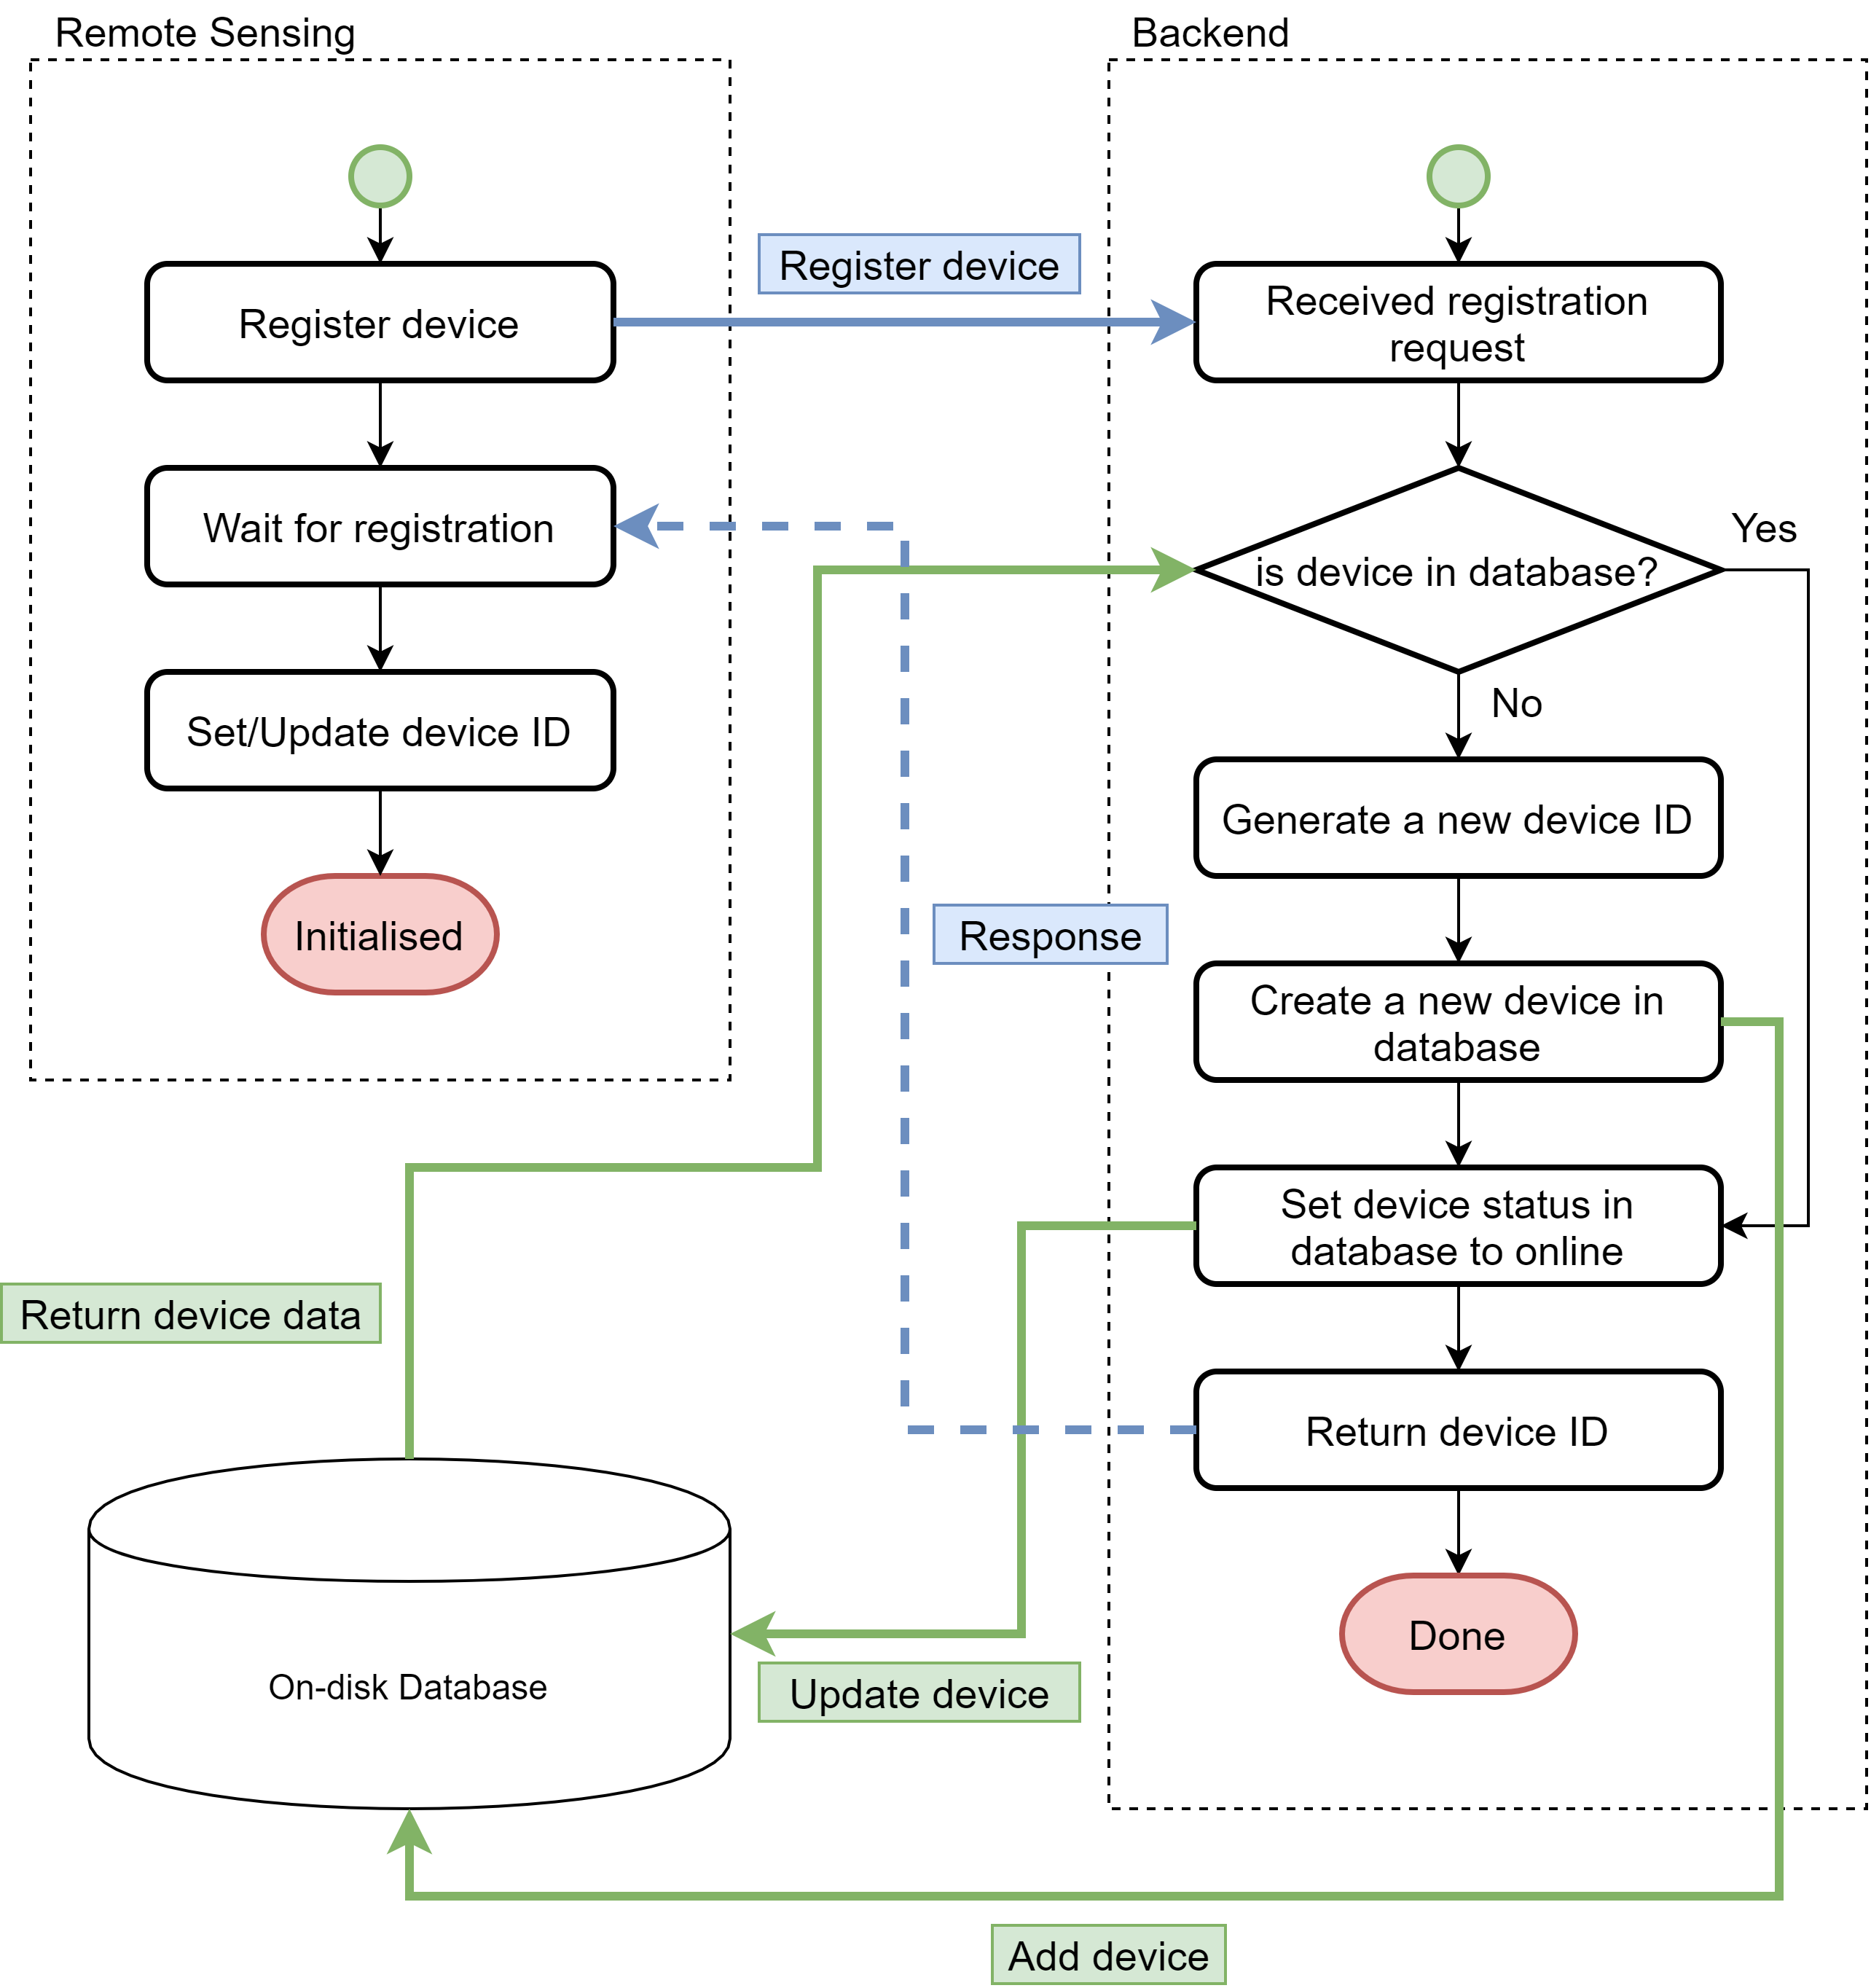
\includegraphics[width=\linewidth]{c4-initialisation.png}
	\caption{The initialisation process.}
	\label{fig:init}
\end{figure}

\subsection{Data recording and device controlling}

The data recording process aims to record data from the sensors and store them into the database. The process begins at the microcontroller where it reads the sensing data from the sensors and then sends it to the backend using the \emph{push new sensing data} request. Once the backend received the sensing data, it begins to execte two sequence of instructions simultaneously. The first sequence is used for data recording, where the data is added to the database and then sends a message to clients notifying a new sensing data is available. The second sequence is used for device controlling, where it retrieves a list of commands cumulated in the database, and sends them to the microcontroller through the response to the \emph{push new sensing data} request. As soon as the microcontroller received the commands, it would perform each command in order and wait for 1 second before reading and sending data again. The process is shown in the figure \ref{fig:record}. 

The reason for data recording and device controlling happening at the same time is improving communication efficiency and reducing server load. The microcontroller doesn't need to send two different requests to push data and retrieve commands, which reduces the communication time by half and reduces the number of access to the backend by half. 

Executing the two seqeunce of instructions simultaneously have the benefit of reducing the response time of a request. 

\begin{figure}[!ht]
	\centering
	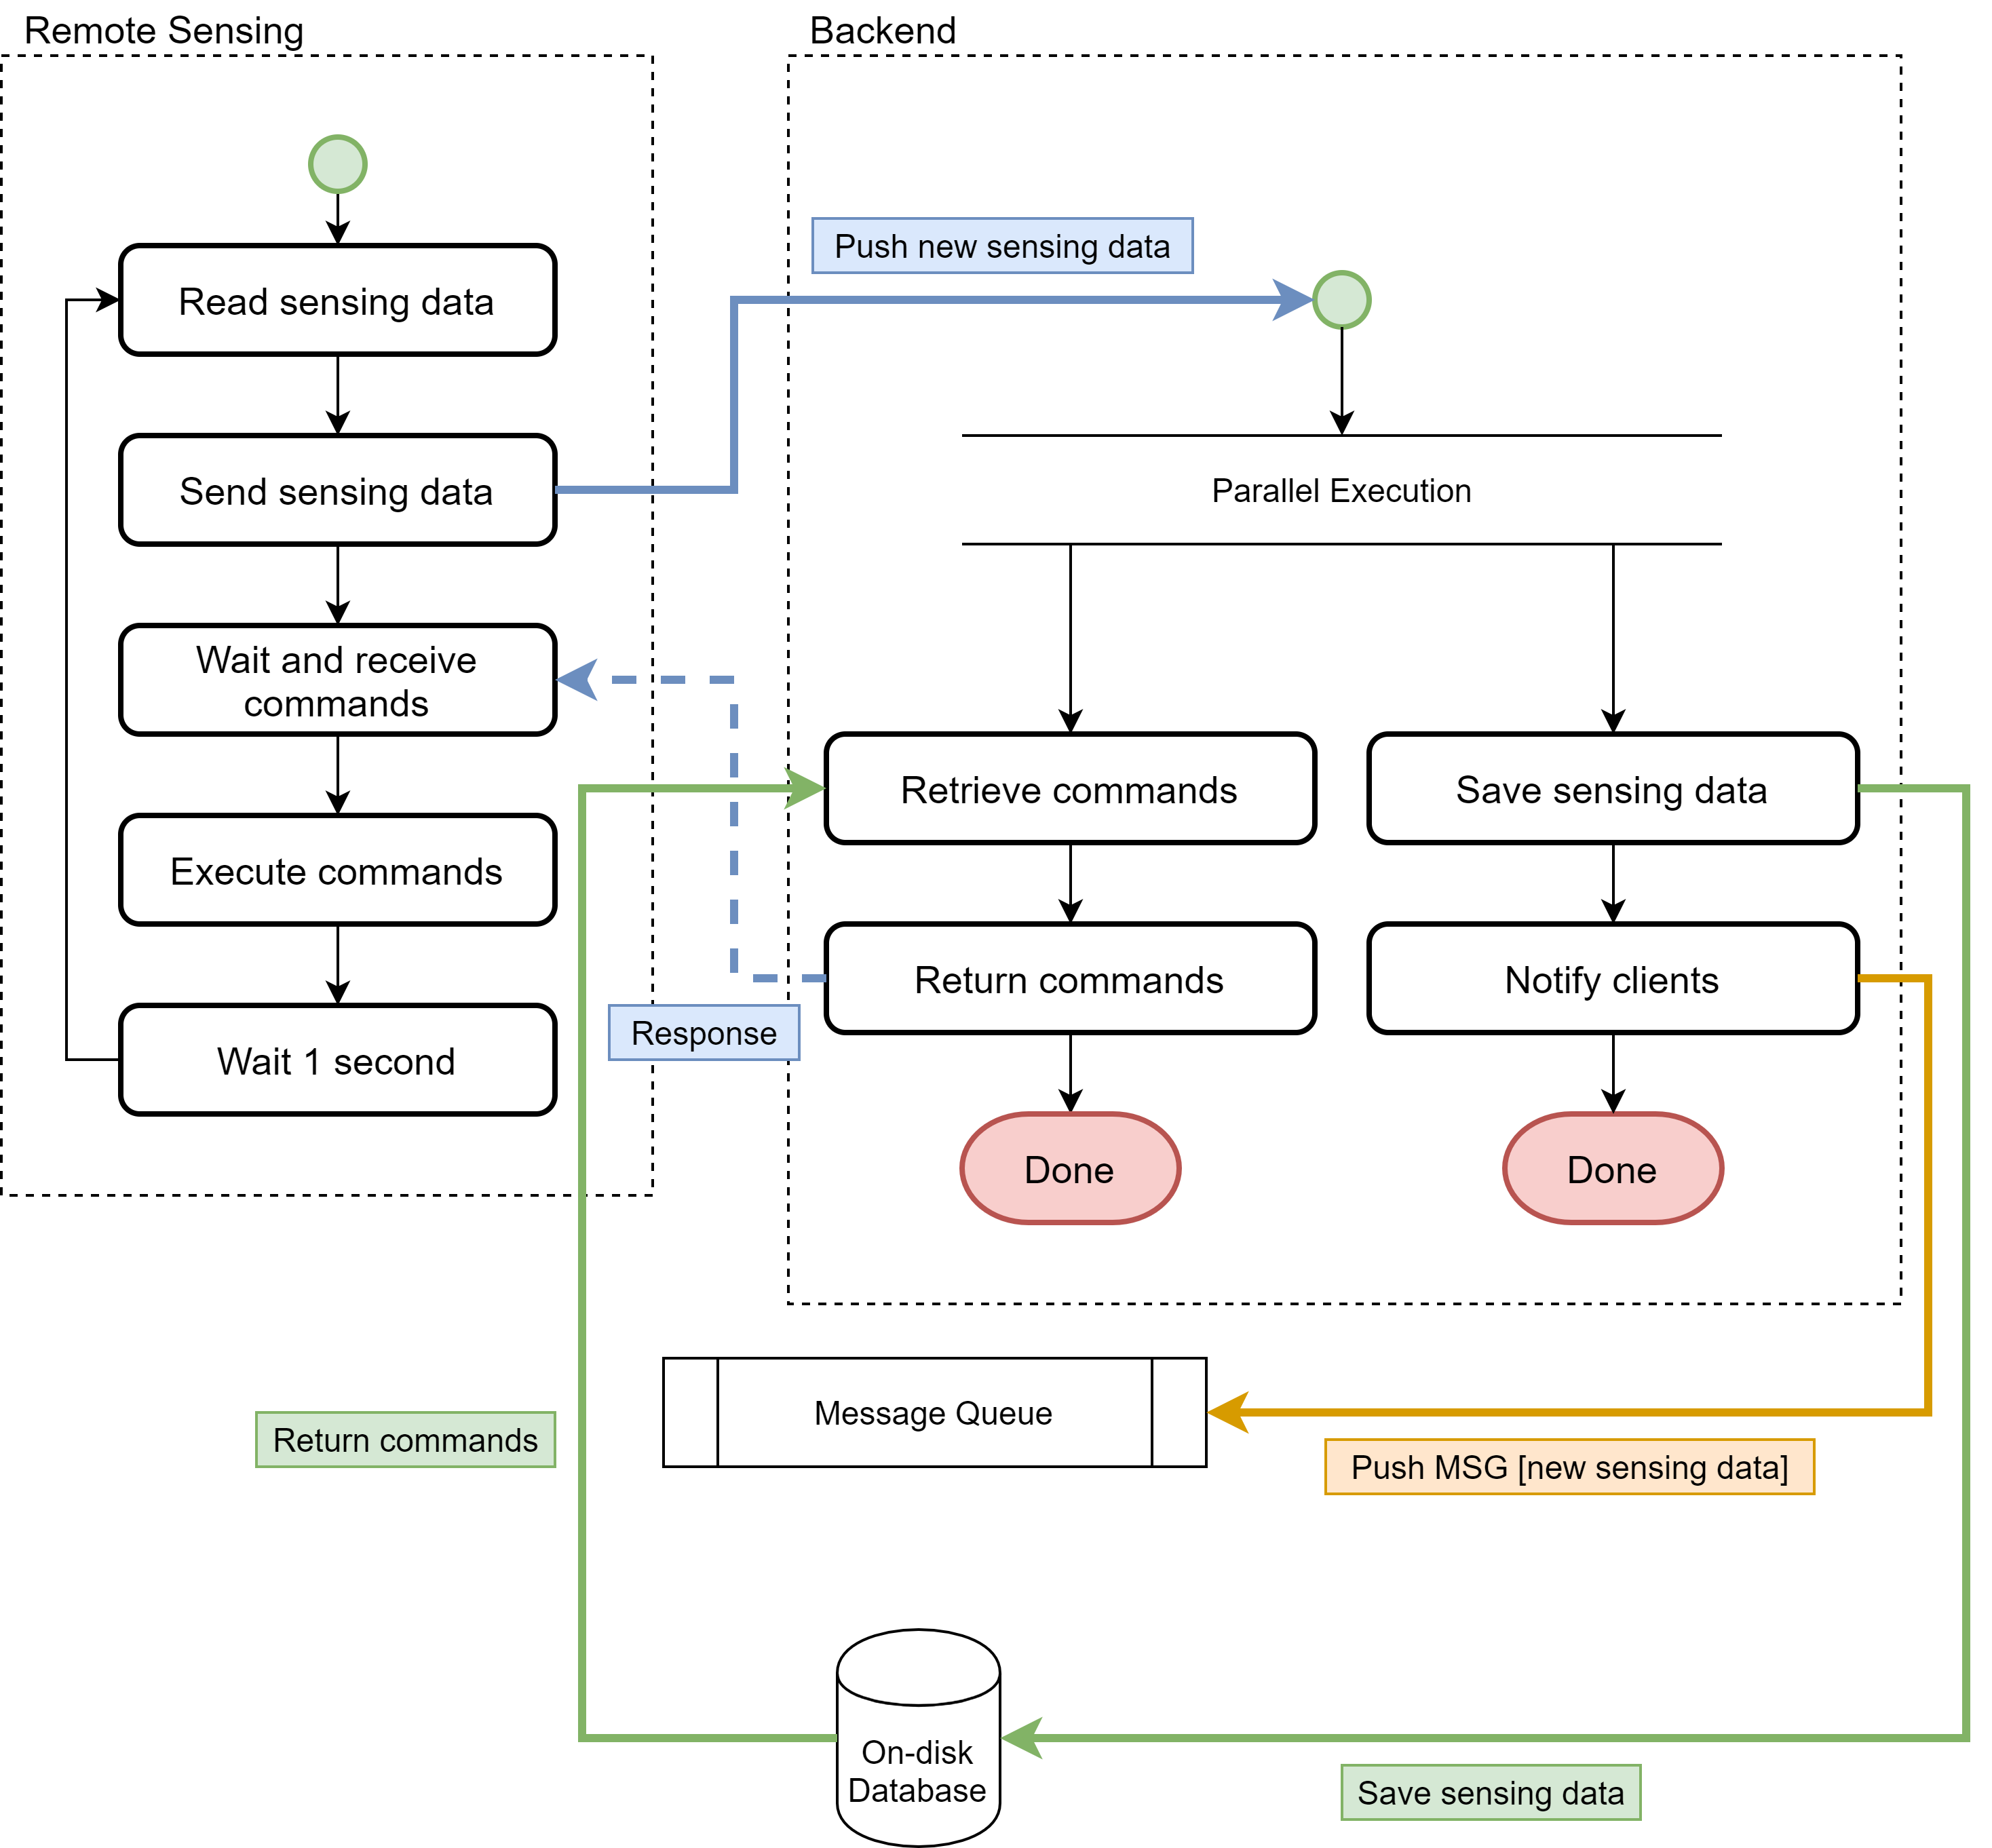
\includegraphics[width=\linewidth]{c4-recording.png}
	\caption{The data recording process.}
	\label{fig:record}
\end{figure}

\subsection{Governing}


\subsection{Context-aware load balancing}

\subsection{Data monitoring}

\subsection{Issuing command}




\newpage
\section{Remote sensing}
\label{sec:remoteSensing}
sdfsdf

\section{Backend}
\label{sec:backend}
sdfsdf
\section{Frontend}
\label{sec:frontend}
sdfsdf
\section{Real-time}
\label{sec:realtime}
sdfsdf
\section{Governor}
\label{sec:governor}
sdfsdf
\section{Simulator}
\label{sec:simulator}
sdfsdf
\section{Client}
\label{sec:webClient}


\end{document}